\section{Figures}
\label{apx:figures}

Images used in these figures fall under the Fair Use doctrine of U.S. Copyright law.

\begin{figure}[ht]
\caption{Autism Speaks Logo}
\centering

\includegraphics[width=0.333\textwidth]{aspeaks}
\label{fig:aspeaks}
\end{figure}

\begin{figure}[ht]
\caption{Twitter Jigsaw Emoji}
\centering

\includegraphics[width=0.2\textwidth]{twitterJigsaw}
\label{fig:twitterJigsaw}
\end{figure}

\begin{figure}[ht]
\caption{Rainbow Infinity Loop}
\centering
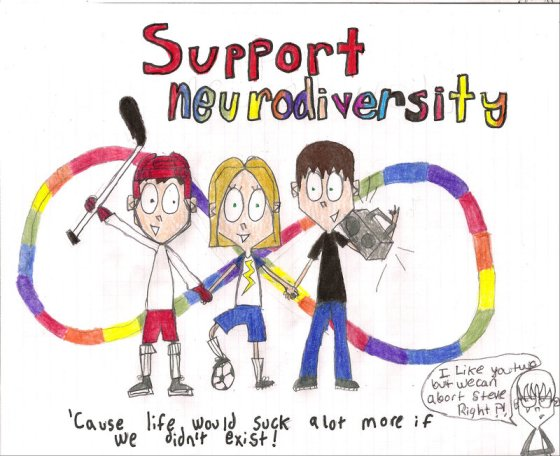
\includegraphics[width=0.5\textwidth]{infinity.jpg}
\label{fig:infinity}
\end{figure}

\begin{figure}[ht]
\caption[Twitter User with Brain Emoji]{Autistic Twitter User with Brain Emoji. Notice the brain on her shirt is rainbow.}
\centering

\includegraphics[width=0.3\textwidth]{rebel.png}
\label{fig:rebel}
\end{figure}

\begin{figure}[ht]
\caption[Twitter User with Puzzle Piece Emoji]{Autistic Twitter User with Puzzle Piece. Personal information about the user intentionally obfuscated.}
\centering
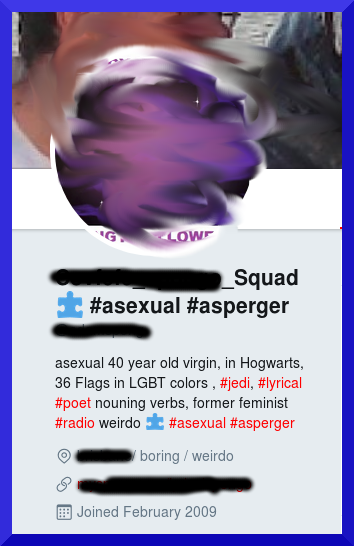
\includegraphics[width=0.3\textwidth]{covfefe.png}
\label{fig:covfefe}
\end{figure}

\begin{figure}[ht]
\caption{Instructive Drawing of Brain using Multiple Colors}
\centering
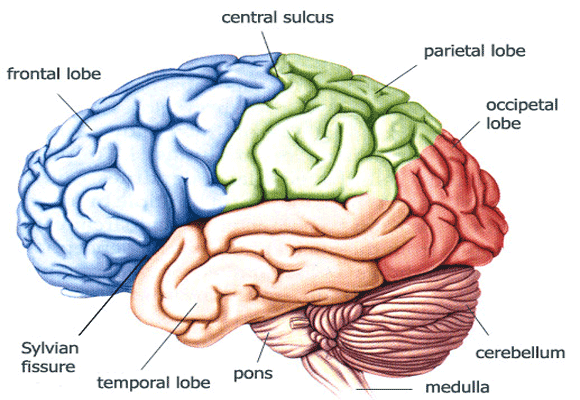
\includegraphics[width=0.5\textwidth]{brainparts.png}
\label{fig:brainparts}
\end{figure}

